%!TEX root =  ../main.tex

\chapterimage{\chapdir/pics/NM_12-06-06_0576_(7175101925)}
\mychapter{Conics}{conics}

Rotated, Eccentricity

\newpage
\chapterminitoc

\newpage
\section{Introduction to Conics}
\noindent\makebox[\textwidth]{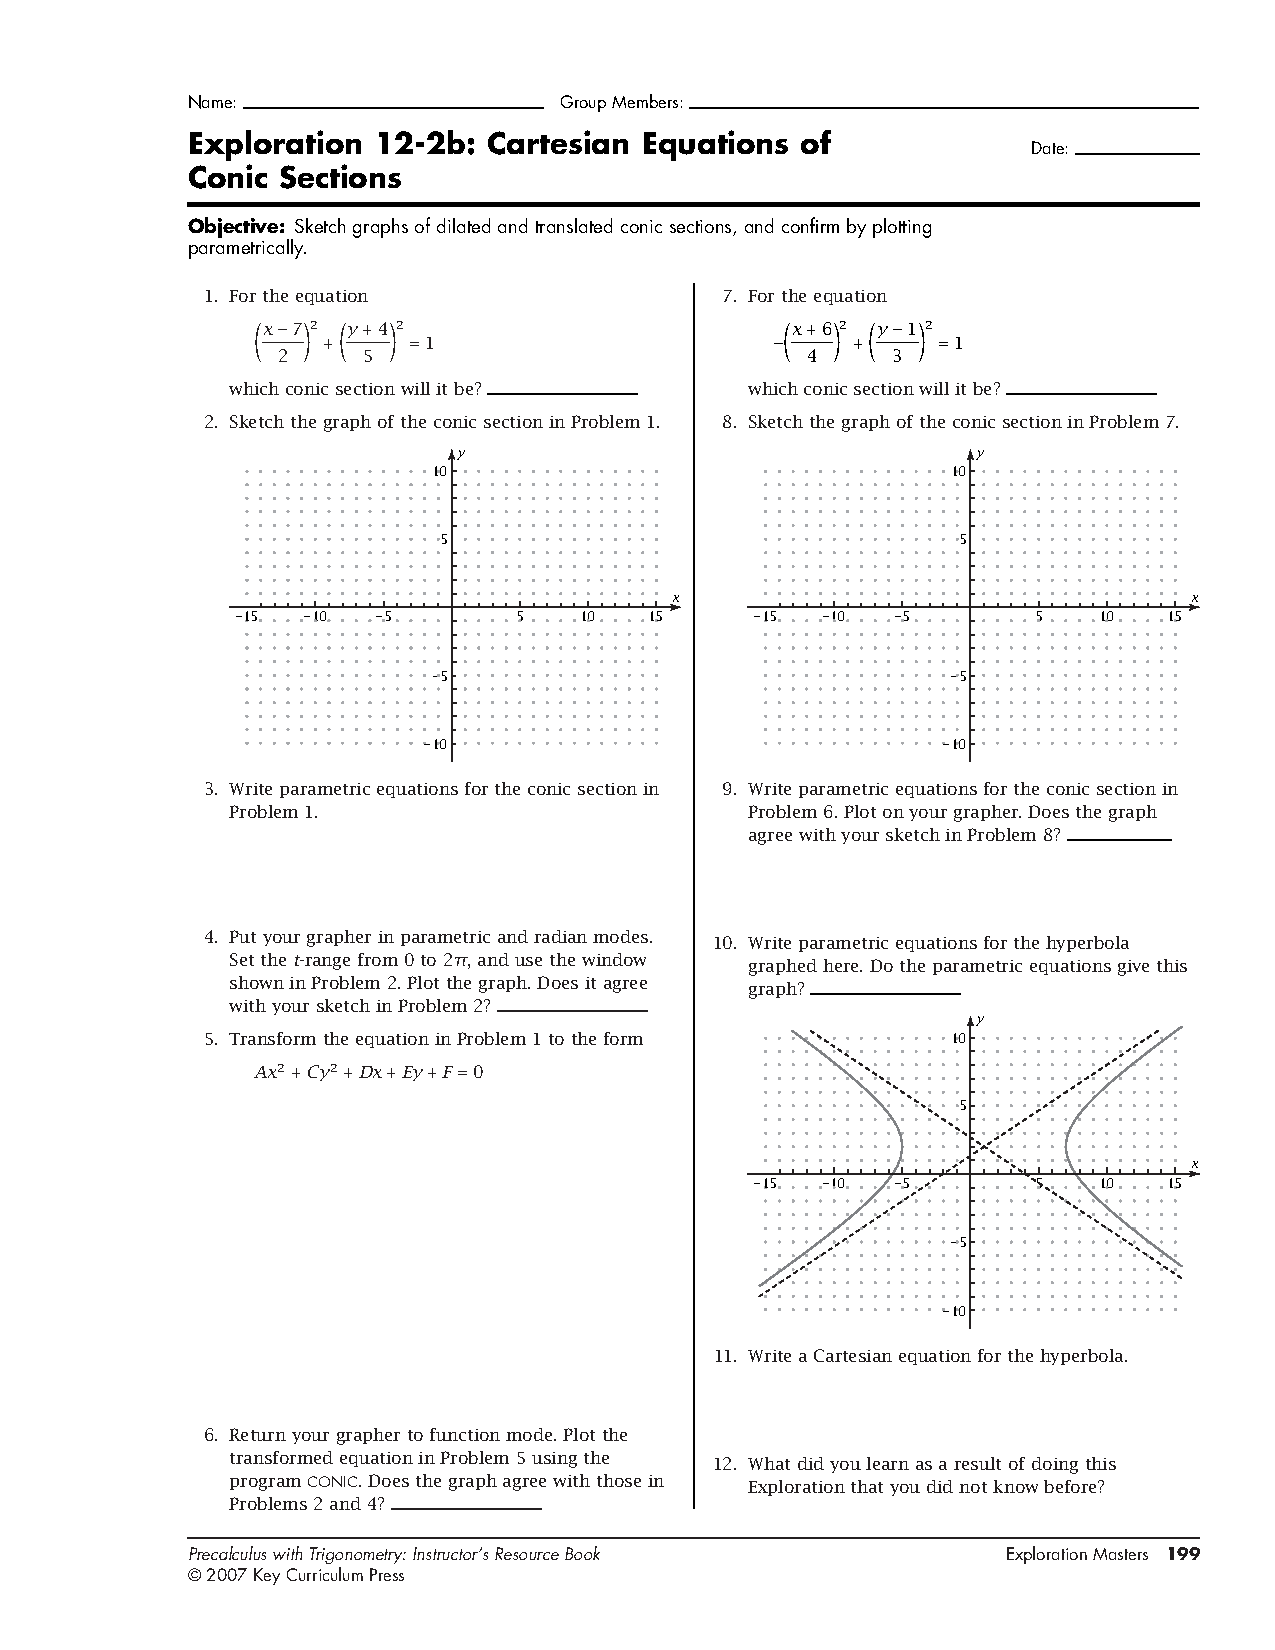
\includegraphics[width=\paperwidth]{chDD/DD01p.pdf}}
\subsection{Graphing form}
of circles, parabolas, ellipses, and hyperbola

\subsection{Algebra General Form}
\subsection{Using a Calculator}

\newpage
\section{Algebra Manipulations}
\noindent\makebox[\textwidth]{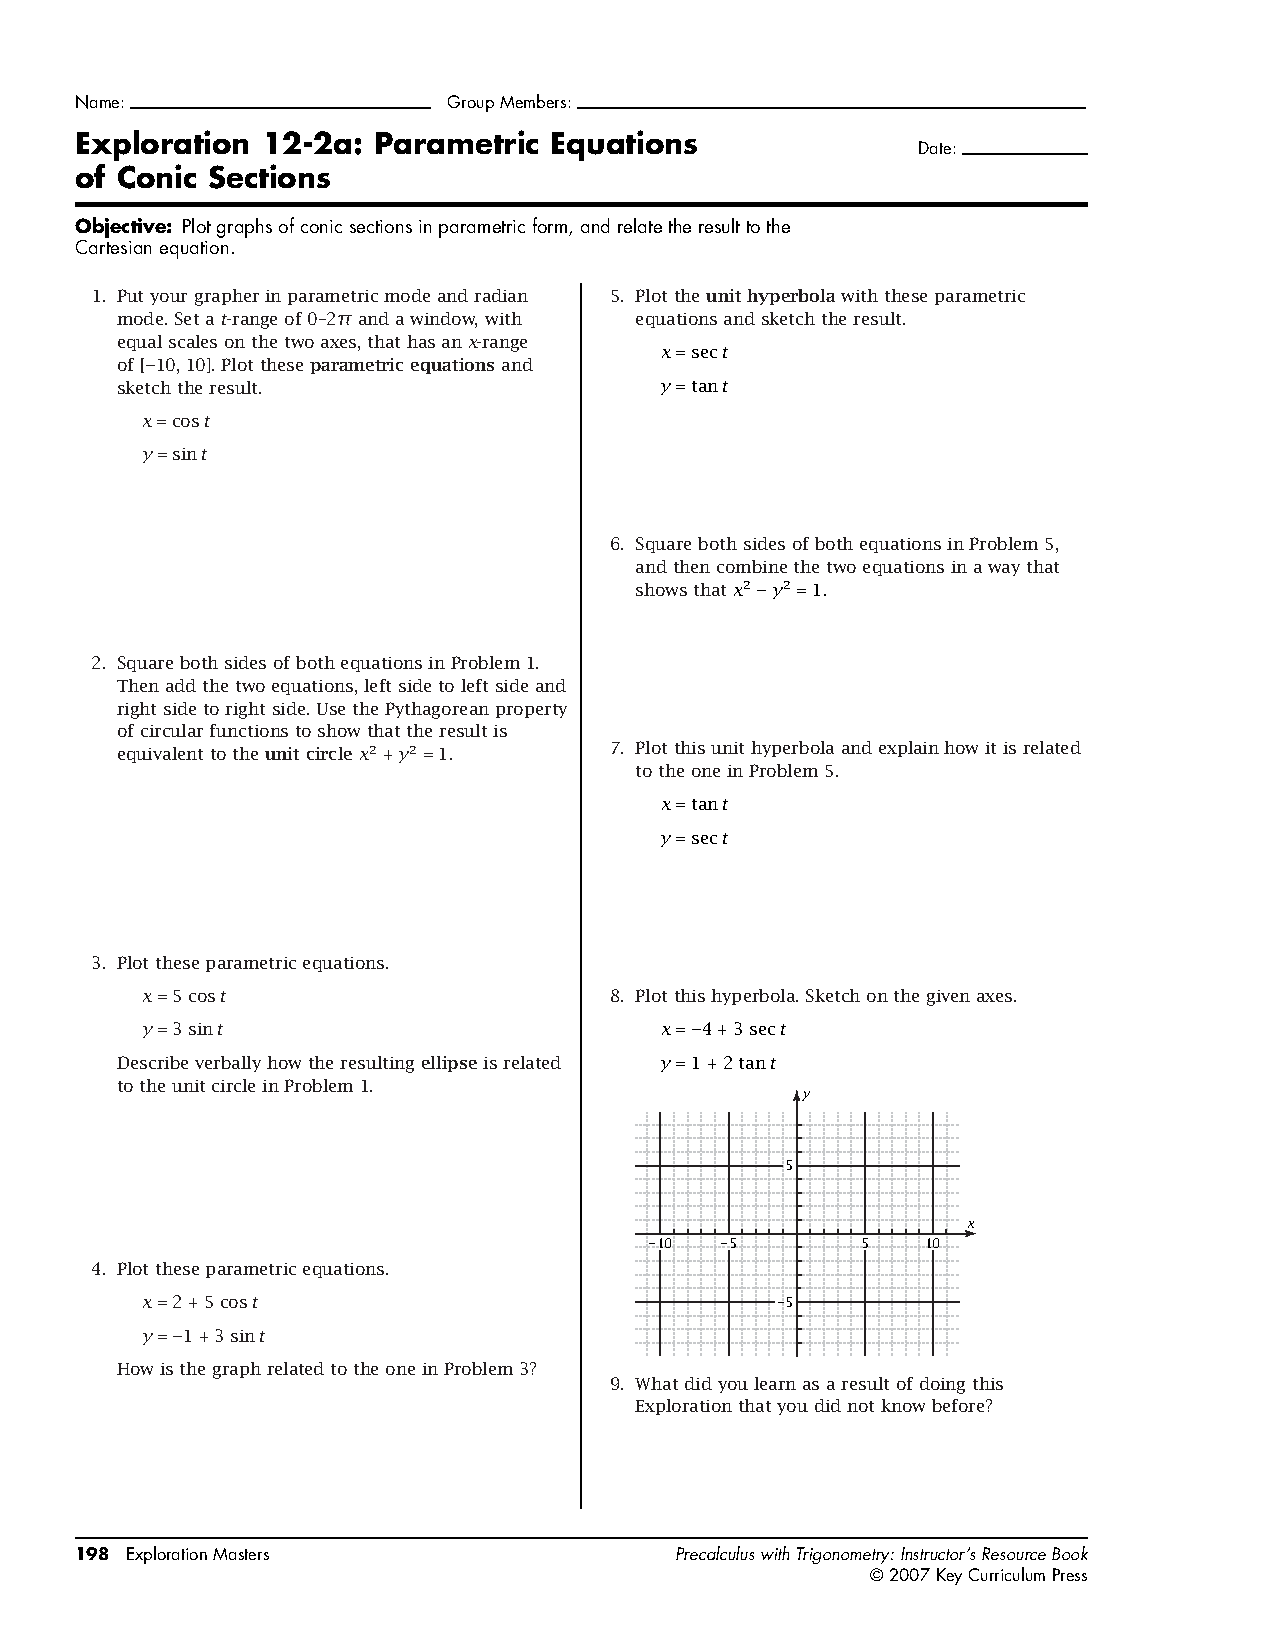
\includegraphics[width=\paperwidth]{chDD/DD02p.pdf}}
\subsection{Discriminant}
\subsection{Completing the Square}
\subsection{Cartesian Forms}
\subsection{Parametric Forms}
\subsection{Polar Forms}

\newpage
\section{Rotated Conics}
\subsection{Rotated Polar Conics}
\subsection{Cartesian Rotation Equations}
\subsection{Parametric Rotation by Matrix}

\newpage
\section{Eccentricity}
\subsection{Range of Eccentricity}
\subsection{Foci}
\subsection{Directrices}
\subsection{Distance Formulae}

\newpage
\section{3D Conics}
\noindent\makebox[\textwidth]{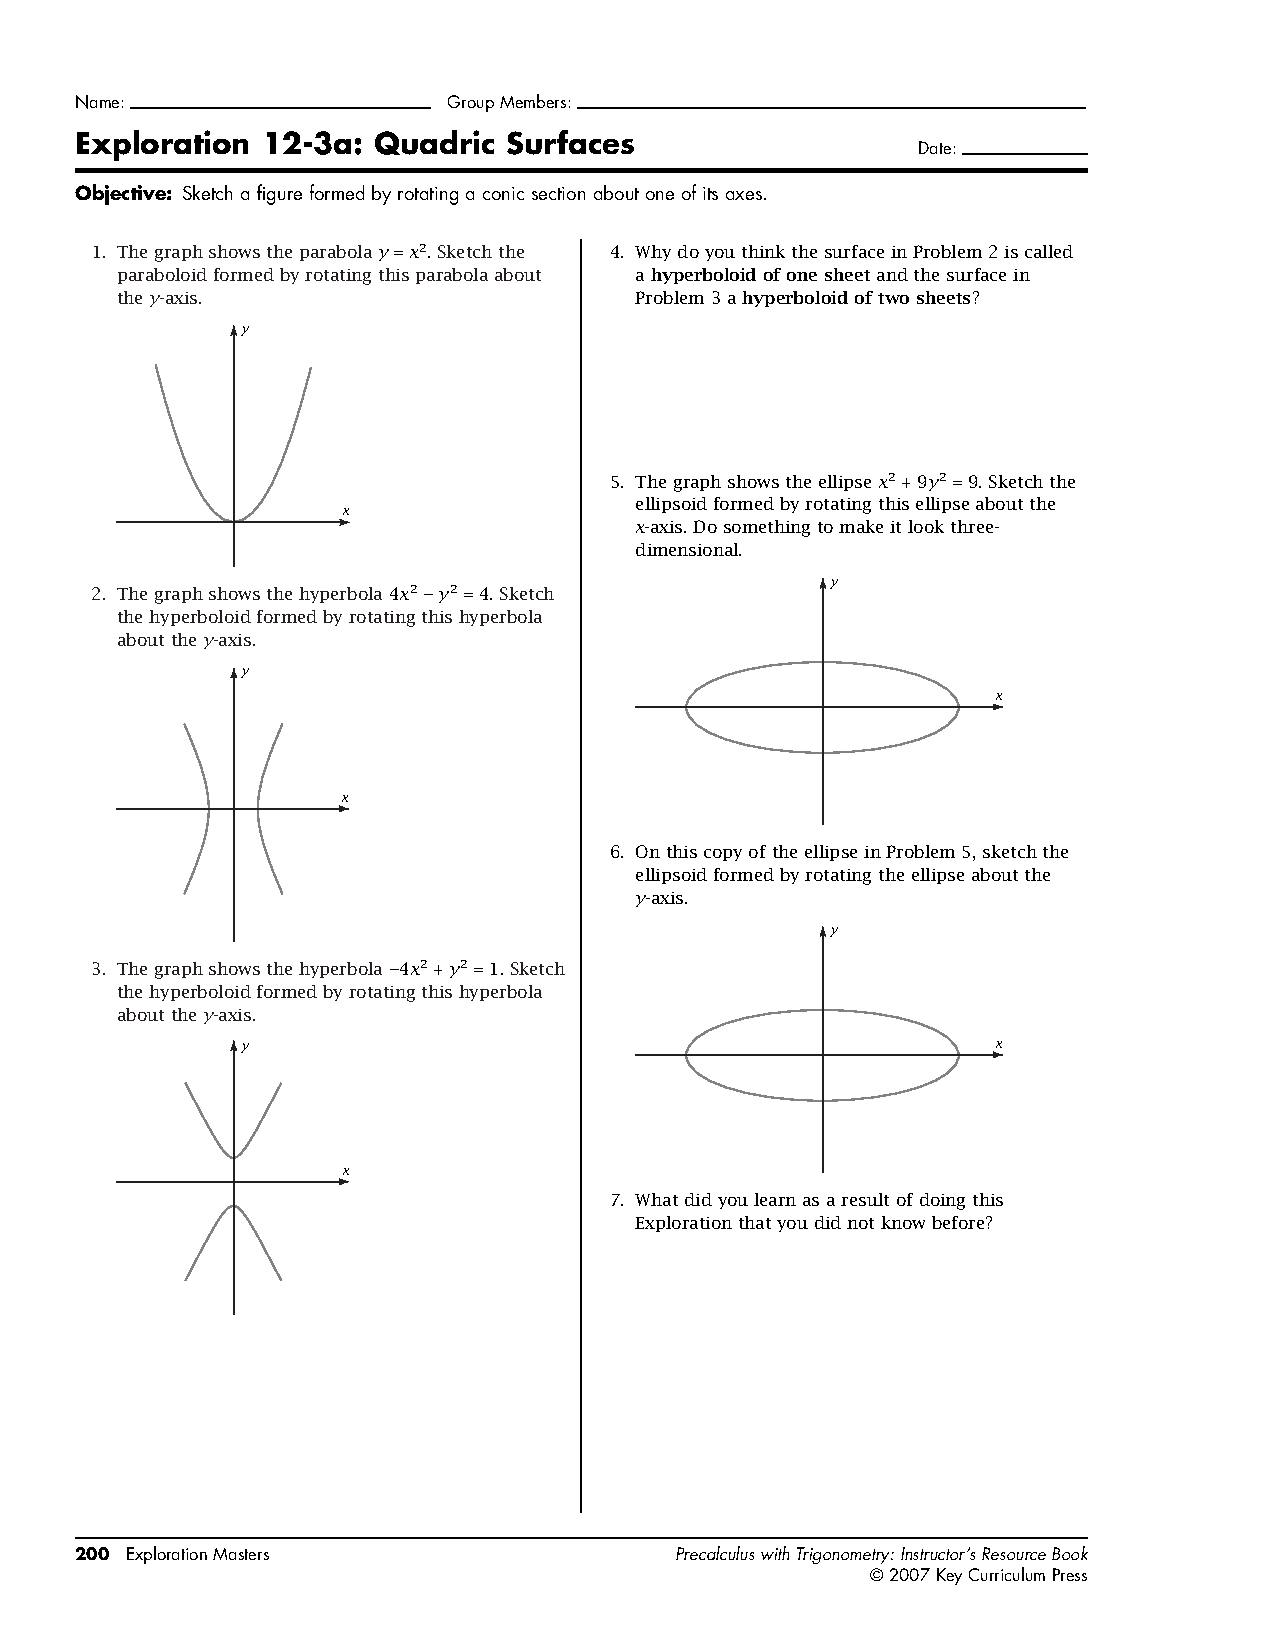
\includegraphics[width=\paperwidth]{chDD/DD05p.pdf}}
\subsection{2.5D}
\subsection{$x, y, z$}
\subsection{$r, \theta, z$}
\subsection{$\rho, \phi, \theta$}

\section{Chapter Review}